\chapter{WF-139 Respecting the Dojo Ratchet To 1796}\label{record-221}

\noindent{\footnotesize\color{BookMuted}\path{docs/design/WF-139-respecting-dojo-ratchet-1796.md}\par}\smallskip

\begin{RecordMeta}
title: WF-139 Respecting the Dojo Ratchet To 1796
legend: WF
lane: bad-code
priority: high
github_issue: 383
status: in_progress
keywords:
  - code-dojo
  - eslint
  - standards
  - ratchet
  - respectful-repo

\end{RecordMeta}

Legend: \href{https://github.com/flyingrobots/bijou/blob/cbd70612140e7a450d764b3c7be1c6af878b99bc/docs/legends/WF-workflow-delivery.md}{WF - Workflow and Delivery}

\section{Linked Work}\label{record-221-linked-work}

\begin{itemize}
\tightlist
\item
  Issue: \href{https://github.com/flyingrobots/bijou/issues/383}{\#383}
\item
  Standards artifact: \href{https://github.com/flyingrobots/bijou/blob/cbd70612140e7a450d764b3c7be1c6af878b99bc/docs/typescript-code-standards.editors-edition.md}{TypeScript Code Standards Editor's Edition}
\item
  Exception ledger: \href{https://github.com/flyingrobots/bijou/blob/cbd70612140e7a450d764b3c7be1c6af878b99bc/docs/code-dojo-exceptions.md}{Code Dojo Exceptions}
\end{itemize}

\section{Decision Summary}\label{record-221-decision-summary}

WF-138 merged with aggregate Code Dojo debt at \texttt{1\allowbreak{},\allowbreak{}8\allowbreak{}4\allowbreak{}6}, including \texttt{1\allowbreak{},\allowbreak{}4\allowbreak{}3\allowbreak{}4} type-aware ESLint findings. The repo goal remains zero ESLint errors, zero Code Dojo issues, and zero files violating length restrictions. The ratchet policy requires every met goalpost to remove at least 50 counted violations until zero.

This cycle targets the next ratchet: lower aggregate debt from \texttt{1\allowbreak{},\allowbreak{}8\allowbreak{}4\allowbreak{}6} to \texttt{1\allowbreak{},\allowbreak{}7\allowbreak{}9\allowbreak{}6} or lower without weakening rules, excluding files, or raising any baseline.

\section{Sponsored Human}\label{record-221-sponsored-human}

A maintainer wants the Dojo loop to keep moving immediately after WF-138 rather than parking a ready burndown on main and letting the next 50 violations linger.

\section{Sponsored Agent}\label{record-221-sponsored-agent}

An agent needs a bounded cluster with enough current ESLint density to clear the next goalpost while keeping touched-file size ratchets flat or lower.

\section{Hill}\label{record-221-hill}

Reduce aggregate Code Dojo debt from \texttt{1\allowbreak{},\allowbreak{}8\allowbreak{}4\allowbreak{}6} to \texttt{1\allowbreak{},\allowbreak{}7\allowbreak{}9\allowbreak{}6} or lower by eliminating at least \texttt{5\allowbreak{}0} live ESLint findings with real fixes.

Final non-DOGFOOD slice from the offender list:

\begin{center}
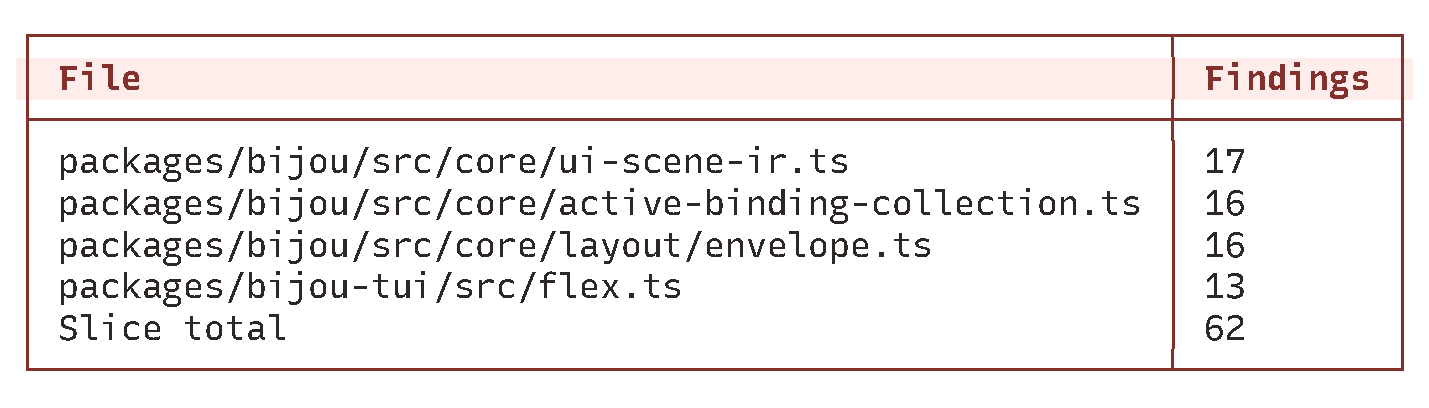
\includegraphics[width=\linewidth]{figures/tables/table-049-g1-1.pdf}
\par\smallskip{\scriptsize\color{BookMuted}Rows 1–5. Actual Bijou table component.}
\end{center}


\section{Implementation Result}\label{record-221-implementation-result}

The final slice lowered live type-aware ESLint findings from \texttt{1\allowbreak{},\allowbreak{}4\allowbreak{}3\allowbreak{}4} to \texttt{1\allowbreak{},\allowbreak{}3\allowbreak{}6\allowbreak{}8} and removed \texttt{p\allowbreak{}a\allowbreak{}c\allowbreak{}k\allowbreak{}a\allowbreak{}g\allowbreak{}e\allowbreak{}s\allowbreak{}/\allowbreak{}b\allowbreak{}i\allowbreak{}j\allowbreak{}o\allowbreak{}u\allowbreak{}-\allowbreak{}t\allowbreak{}u\allowbreak{}i\allowbreak{}/\allowbreak{}s\allowbreak{}r\allowbreak{}c\allowbreak{}/\allowbreak{}f\allowbreak{}l\allowbreak{}e\allowbreak{}x\allowbreak{}.\allowbreak{}t\allowbreak{}s} from the code-size baseline by shrinking it to the 500-line ratchet boundary. Aggregate Code Dojo debt fell from \texttt{1\allowbreak{},\allowbreak{}8\allowbreak{}4\allowbreak{}6} to \texttt{1\allowbreak{},\allowbreak{}7\allowbreak{}7\allowbreak{}9}.

\section{Scope}\label{record-221-scope}

\begin{itemize}
\tightlist
\item
  Replace non-null assertions and unsafe assertions with checked reads, structural guards, or narrowed helper functions.
\item
  Make template interpolation explicit where values are not statically strings.
\item
  Remove stale or redundant conditionals only when behavior is preserved.
\item
  Keep UI scene IR hashing/lowering, active-binding collection behavior, layout envelope negotiation, and TUI flex behavior stable.
\item
  Lower \texttt{s\allowbreak{}c\allowbreak{}r\allowbreak{}i\allowbreak{}p\allowbreak{}t\allowbreak{}s\allowbreak{}/\allowbreak{}c\allowbreak{}o\allowbreak{}d\allowbreak{}e\allowbreak{}-\allowbreak{}d\allowbreak{}o\allowbreak{}j\allowbreak{}o\allowbreak{}/\allowbreak{}b\allowbreak{}a\allowbreak{}s\allowbreak{}e\allowbreak{}l\allowbreak{}i\allowbreak{}n\allowbreak{}e\allowbreak{}s\allowbreak{}/\allowbreak{}e\allowbreak{}s\allowbreak{}l\allowbreak{}i\allowbreak{}n\allowbreak{}t\allowbreak{}.\allowbreak{}j\allowbreak{}s\allowbreak{}o\allowbreak{}n}, \texttt{d\allowbreak{}o\allowbreak{}c\allowbreak{}s\allowbreak{}/\allowbreak{}c\allowbreak{}o\allowbreak{}d\allowbreak{}e\allowbreak{}-\allowbreak{}d\allowbreak{}o\allowbreak{}j\allowbreak{}o\allowbreak{}-\allowbreak{}e\allowbreak{}x\allowbreak{}c\allowbreak{}e\allowbreak{}p\allowbreak{}t\allowbreak{}i\allowbreak{}o\allowbreak{}n\allowbreak{}s\allowbreak{}.\allowbreak{}m\allowbreak{}d}, and \texttt{p\allowbreak{}a\allowbreak{}c\allowbreak{}k\allowbreak{}a\allowbreak{}g\allowbreak{}e\allowbreak{}.\allowbreak{}j\allowbreak{}s\allowbreak{}o\allowbreak{}n} only after live counts prove the reduction.
\end{itemize}

\section{Non-Goals}\label{record-221-non-goals}

\begin{itemize}
\tightlist
\item
  Weakening ESLint rules, Code Dojo thresholds, or standards artifacts is out of scope.
\item
  File/context and code-size ceilings must not rise.
\item
  Unrelated rendering or layout architecture refactors are out of scope.
\item
  Exception churn cannot stand in for real cleanup.
\end{itemize}

\section{Current Evidence}\label{record-221-current-evidence}

Live counts on \texttt{m\allowbreak{}a\allowbreak{}i\allowbreak{}n} at \texttt{f\allowbreak{}8\allowbreak{}2\allowbreak{}0\allowbreak{}f\allowbreak{}c\allowbreak{}0\allowbreak{}7}:

\begin{itemize}
\tightlist
\item
  aggregate Code Dojo debt: \texttt{1\allowbreak{},\allowbreak{}8\allowbreak{}4\allowbreak{}6}
\item
  ESLint findings: \texttt{1\allowbreak{},\allowbreak{}4\allowbreak{}3\allowbreak{}4}
\item
  file/context baseline: \texttt{3\allowbreak{}3\allowbreak{}3}
\item
  mock-ban baseline: \texttt{2\allowbreak{}3}
\item
  code-size baseline: \texttt{5\allowbreak{}6}, including \texttt{4} legacy hard-limit files
\item
  next aggregate target: \texttt{1\allowbreak{},\allowbreak{}7\allowbreak{}9\allowbreak{}6} or lower
\end{itemize}

Live counts after the implementation slice:

\begin{itemize}
\tightlist
\item
  aggregate Code Dojo debt: \texttt{1\allowbreak{},\allowbreak{}7\allowbreak{}7\allowbreak{}9}
\item
  ESLint findings: \texttt{1\allowbreak{},\allowbreak{}3\allowbreak{}6\allowbreak{}8}
\item
  file/context baseline: \texttt{3\allowbreak{}3\allowbreak{}3}
\item
  mock-ban baseline: \texttt{2\allowbreak{}3}
\item
  code-size baseline: \texttt{5\allowbreak{}5}, including \texttt{4} legacy hard-limit files
\item
  next aggregate target: \texttt{1\allowbreak{},\allowbreak{}7\allowbreak{}2\allowbreak{}9} or lower
\end{itemize}

\section{Playback Questions}\label{record-221-playback-questions}

\begin{enumerate}
\def\labelenumi{\arabic{enumi}.}
\tightlist
\item
  Is aggregate Code Dojo debt at \texttt{1\allowbreak{},\allowbreak{}7\allowbreak{}9\allowbreak{}6} or lower?
\item
  Does the stored ESLint baseline match the new live count?
\item
  Have file/context and code-size debt held or shrunk?
\item
  Do focused tests for the touched surfaces pass?
\item
  Are the repo gates passing before review?
\end{enumerate}

\section{Tests To Write First}\label{record-221-tests-to-write-first}

The lint findings are the RED signal for pure type-safety rewrites. Add focused regression tests before changing behavior in UI scene lowering, active binding, layout envelope resolution, or flex layout.

\section{Acceptance Criteria}\label{record-221-acceptance-criteria}

\begin{itemize}
\tightlist
\item
  The selected touched TypeScript files have zero new ESLint findings and reduce live findings by at least \texttt{5\allowbreak{}0}.
\item
  Aggregate Code Dojo debt is \texttt{1\allowbreak{},\allowbreak{}7\allowbreak{}7\allowbreak{}9} or lower.
\item
  \texttt{s\allowbreak{}c\allowbreak{}r\allowbreak{}i\allowbreak{}p\allowbreak{}t\allowbreak{}s\allowbreak{}/\allowbreak{}c\allowbreak{}o\allowbreak{}d\allowbreak{}e\allowbreak{}-\allowbreak{}d\allowbreak{}o\allowbreak{}j\allowbreak{}o\allowbreak{}/\allowbreak{}b\allowbreak{}a\allowbreak{}s\allowbreak{}e\allowbreak{}l\allowbreak{}i\allowbreak{}n\allowbreak{}e\allowbreak{}s\allowbreak{}/\allowbreak{}e\allowbreak{}s\allowbreak{}l\allowbreak{}i\allowbreak{}n\allowbreak{}t\allowbreak{}.\allowbreak{}j\allowbreak{}s\allowbreak{}o\allowbreak{}n} records the lower live ESLint count.
\item
  \texttt{d\allowbreak{}o\allowbreak{}c\allowbreak{}s\allowbreak{}/\allowbreak{}c\allowbreak{}o\allowbreak{}d\allowbreak{}e\allowbreak{}-\allowbreak{}d\allowbreak{}o\allowbreak{}j\allowbreak{}o\allowbreak{}-\allowbreak{}e\allowbreak{}x\allowbreak{}c\allowbreak{}e\allowbreak{}p\allowbreak{}t\allowbreak{}i\allowbreak{}o\allowbreak{}n\allowbreak{}s\allowbreak{}.\allowbreak{}m\allowbreak{}d} and \texttt{p\allowbreak{}a\allowbreak{}c\allowbreak{}k\allowbreak{}a\allowbreak{}g\allowbreak{}e\allowbreak{}.\allowbreak{}j\allowbreak{}s\allowbreak{}o\allowbreak{}n} report the lower ceiling.
\item
  Focused validation for the touched surfaces passes.
\item
  \texttt{n\allowbreak{}p\allowbreak{}m\allowbreak{} \allowbreak{}r\allowbreak{}u\allowbreak{}n\allowbreak{} \allowbreak{}c\allowbreak{}o\allowbreak{}d\allowbreak{}e\allowbreak{}-\allowbreak{}d\allowbreak{}o\allowbreak{}j\allowbreak{}o\allowbreak{}:\allowbreak{}v\allowbreak{}e\allowbreak{}r\allowbreak{}i\allowbreak{}f\allowbreak{}y}, \texttt{n\allowbreak{}p\allowbreak{}m\allowbreak{} \allowbreak{}r\allowbreak{}u\allowbreak{}n\allowbreak{} \allowbreak{}d\allowbreak{}o\allowbreak{}c\allowbreak{}s\allowbreak{}:\allowbreak{}i\allowbreak{}n\allowbreak{}v\allowbreak{}e\allowbreak{}n\allowbreak{}t\allowbreak{}o\allowbreak{}r\allowbreak{}y}, \texttt{n\allowbreak{}p\allowbreak{}m\allowbreak{} \allowbreak{}r\allowbreak{}u\allowbreak{}n\allowbreak{} \allowbreak{}l\allowbreak{}i\allowbreak{}n\allowbreak{}t}, and \texttt{g\allowbreak{}i\allowbreak{}t\allowbreak{} \allowbreak{}d\allowbreak{}i\allowbreak{}f\allowbreak{}f\allowbreak{} \allowbreak{}-\allowbreak{}-\allowbreak{}c\allowbreak{}h\allowbreak{}e\allowbreak{}c\allowbreak{}k} pass before review.
\end{itemize}

